
\chapter{Kernel Density Estimates}
%\chaptermark{EM algorithm}
\HRule \\[-0.5cm] % Horizontal line


%----------------------------------------------------------------------------------------
%	SECTIONS
%---------------------------------------------------------------------------------------
\begin{spacing}{1.5}
%\begin{document}

\section{Kernel Density Estimates}


%\document{Kernel Density Estimates}
%\HRule \\[-0.5cm]

%\begin{spacing}[1.5]
 Kernel Density Estimation (KDE) is a non-parametric way to estimate the probability density function of a random variable.Kernel density estimation is a fundamental data smoothing problem where inferences about the population are made, based on a finite data sample.Kernel Density Estimation is also called Parzen Window.The Parzen-window approach to estimating densities can be introduced by temporarily
assuming that the region $R_{n}$ is a $d$-dimensional hypercube. If $h_{n}$ is the length of an edge of that hypercube, then its volume is given by
                                                  
                                                  
                                                 $V_{n}$=$h_{n}^{d}$
We can obtain an analytic expression for $k_{n}$, the number of samples falling in the window hypercube, by defining the following window function~\cite{parzenwindow}.
\begin{equation}
\varphi(\mathbf{u})=\left\{\begin{array}{ll}
1 & \left|u_{j}\right| \leq 1 / 2 \\
0 & \text { otherwise. }
\end{array} \quad j \neq 1, \ldots, d\right.
\end{equation}
Thus, $\varphi(u)$ defines a unit hypercube centered at the origin. It follows that $\varphi\left(\frac{x-x_{i}}{h_{n}}\right)$ is equal to unity if $x_{i}$ falls within the hypercube of volume $V_{n}$ centered at $x$, and is zero otherwise. The number of samples in this hypercube is therefore given by
\begin{equation}
k_{n}=\sum_{i=1}^{n} \varphi\left(\frac{x-x_{i}}{h_{n}}\right)
\end{equation}
\begin{equation}
p_{n}(\mathbf{x})=\frac{1}{n} \sum_{i=1}^{n} \frac{1}{V_{n}} \varphi\left(\frac{\mathbf{x}-\mathbf{x}{i}}{h_{n}}\right)
\end{equation}
In this Parzen window method, we are going to Estimate the Gaussian univarient and multivariate probability density function with different window sizes.
A Univariate Gaussion Kernel is
\begin{equation}
\varphi_{h}(u)=\frac{1}{\sqrt{2 \pi}} \exp \left[-\frac{1}{2} u^{2}\right]
\end{equation}
The resulting density is given by
\begin{equation}
p(x)=\frac{1}{n} \sum_{i=1}^{n} \frac{1}{h_{n} \sqrt{2 \pi}} \exp \left[-\frac{1}{2 h_{n}^{2}}\left(\mathrm{x}-\mathrm{x}_{i}\right)^{2}\right]
\end{equation}
It shows Parzen-window estimates of a univariate gaussian density using different window widths and number of samples. Here's the figure that I got from my MATLAB code. especially for $n$= 10, 100, 10000 with different window width $h_{1}$= 1, 0.5, 0.2
\section{Results}
\begin{figure}[h]
\label{fig:Parzen window }
  \centering
  {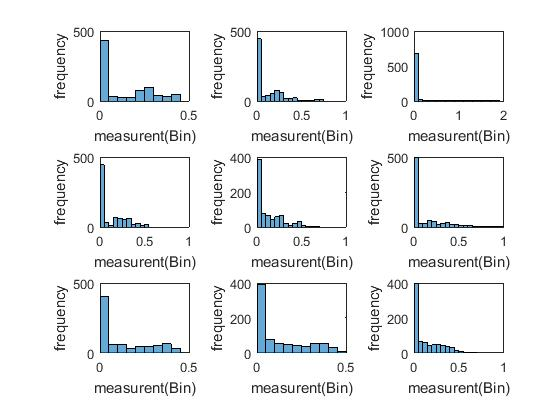
\includegraphics[scale=.7]{Images/histogram of parzen window.jpg} }
  \caption{Histogram of Parzen window estimation for different window sizes.}
\end{figure}

\begin{figure}[h]
\label{fig:Parzen window }
  \centering
  {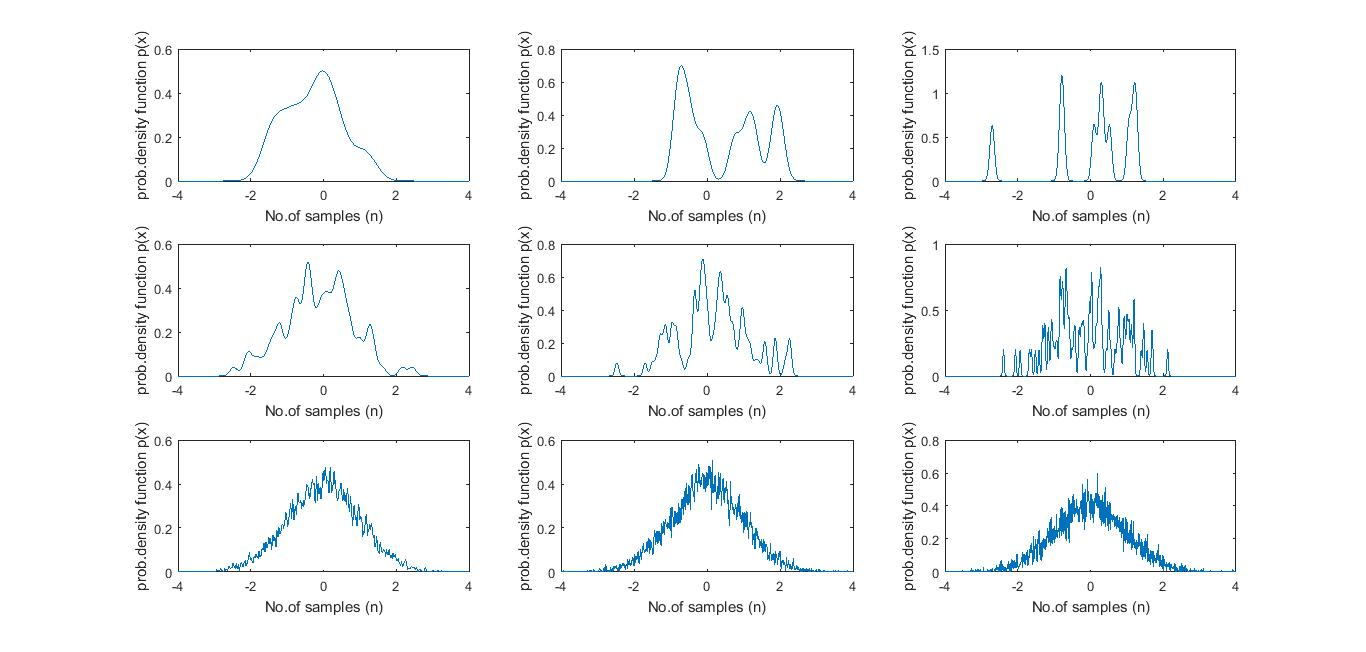
\includegraphics[scale=.38]{Images/parzen window(univarient).jpg} }
  \caption{Parzen window estimation for different window sizes.}
\end{figure}

%\end{spacing}
%\end{document}{}

\end{spacing} 